\documentclass[aspectratio=169]{beamertmd}

\usepackage{graphicx}
\usepackage{tikz}

\title{Wave-Based Modeling for Jointed Structures}
\author{Nidish Narayanaa Balaji}

\begin{document}
\maketitle{}

\begin{frame}[allowframebreaks]
  \frametitle{Dispersion of the Timoshenko Beam}
  \vspace{-0.5cm}\begin{figure}[!h]
    \centering
    \includegraphics[height=2cm]{FIGS/CSYS}
  \end{figure}      
  \begin{itemize}
  \item The coordinate systems that will be used here are given in the
    figure above. The beam is taken to be in the XY plane and the
    degrees of freedom for each point on the beam are taken to be
    the displacements $u_x$, $u_y$, and rotation $\theta_z$.
  \item The equations of motion used for the Timoshenko beam are:
    {\tiny
      \begin{align*}
        \begin{bmatrix} \rho A & 0 & 0\\ 0 & \rho A & 0\\0 & 0 & \rho
          I_z \end{bmatrix} \frac{\partial^2}{\partial
                                                                 t^2}\begin{Bmatrix}
                                                                 u_x\\
                                                                 u_y\\\theta_z \end{Bmatrix}
        - \begin{bmatrix} EA & 0 & 0\\ 0 & GA & 0\\0 & 0 &
          EI_z \end{bmatrix} \frac{\partial^2}{\partial
                                                           x^2} \begin{Bmatrix}
                                                           u_x\\u_y\\\theta_z \end{Bmatrix}
        + \begin{bmatrix} 0 & 0 & 0\\ 0 & 0 & GA \\ 0 & -GA &
          0 \end{bmatrix} \frac{\partial}{\partial x}\begin{Bmatrix}
          u_x\\u_y\\\theta_z \end{Bmatrix} + \begin{bmatrix} 0 & 0 & 0
          \\ 0 & 0 & 0 \\ 0 & 0 & GA \end{bmatrix} \begin{Bmatrix}
          u_x\\ u_y\\\theta_z \end{Bmatrix} = \begin{Bmatrix} f_x\\
          f_y\\ m_z\end{Bmatrix}. 
      \end{align*}}
    \pagebreak
  \item Dispersion relationships will be discussed using the wave
    representation $\bar{u} = \bar{U} e^{i(\kappa x-\omega t)}$. 
  \item The dispersion relationship for the axial vibration
    (longitudinal waves) is
    $$ \omega = \sqrt{\frac{E}{\rho}} \kappa $$
  \item For bending vibration (transverse waves), the dispersion
    relationship is
    $$ (\rho^2AI_z)\omega^4 - \left[\rho GA^2+\kappa^2\rho
      AI_z(G+E)\right] \omega^2 + (EGAI_z) \kappa^4 = 0 $$
    \pagebreak
  \item The dispersion relationship is presented below graphically:
    \begin{figure}[!h]
      \centering
      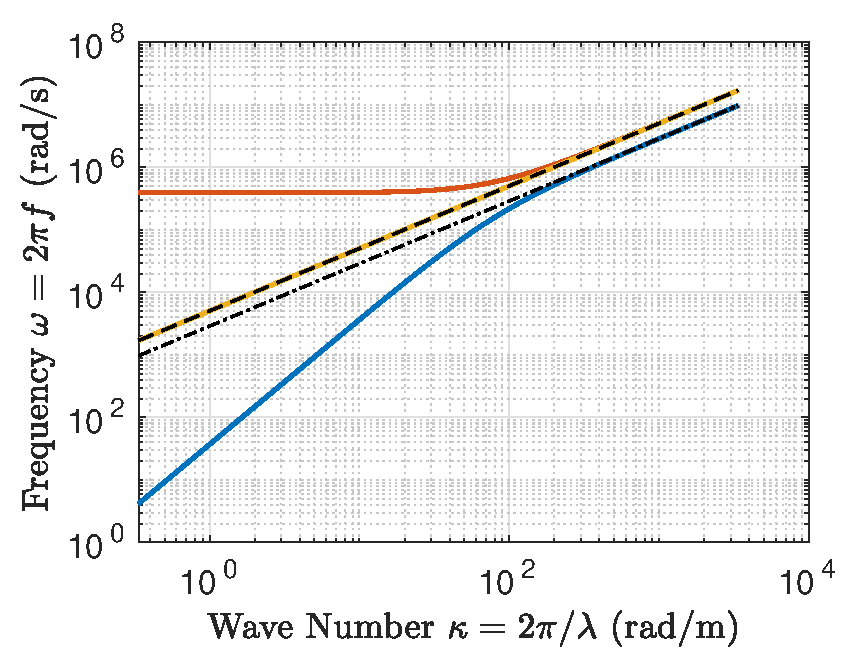
\includegraphics[width=0.35\linewidth]{../../PLANARMODEL/FIGS/TMWS_WvK}%
      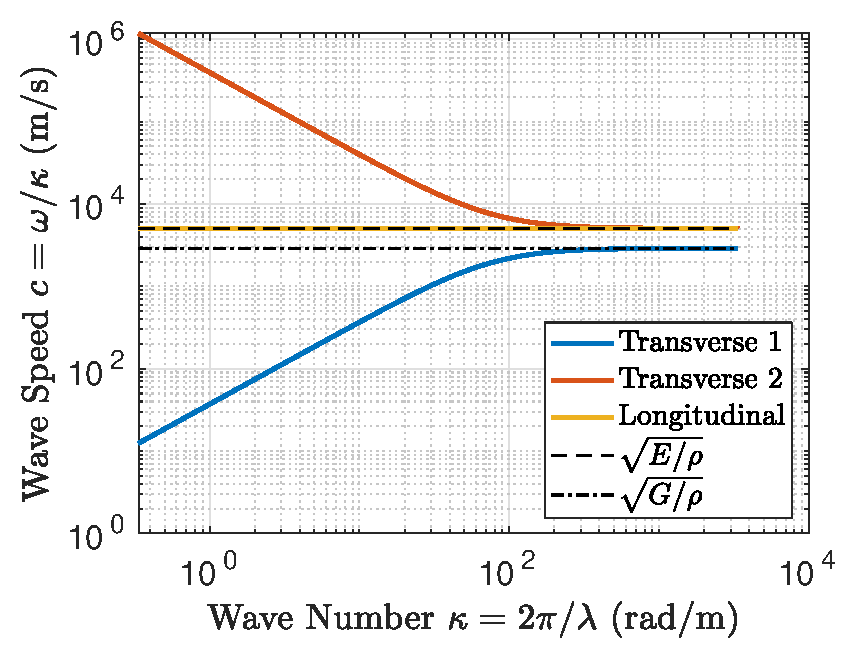
\includegraphics[width=0.35\linewidth]{../../PLANARMODEL/FIGS/TMWS_CvK}%
      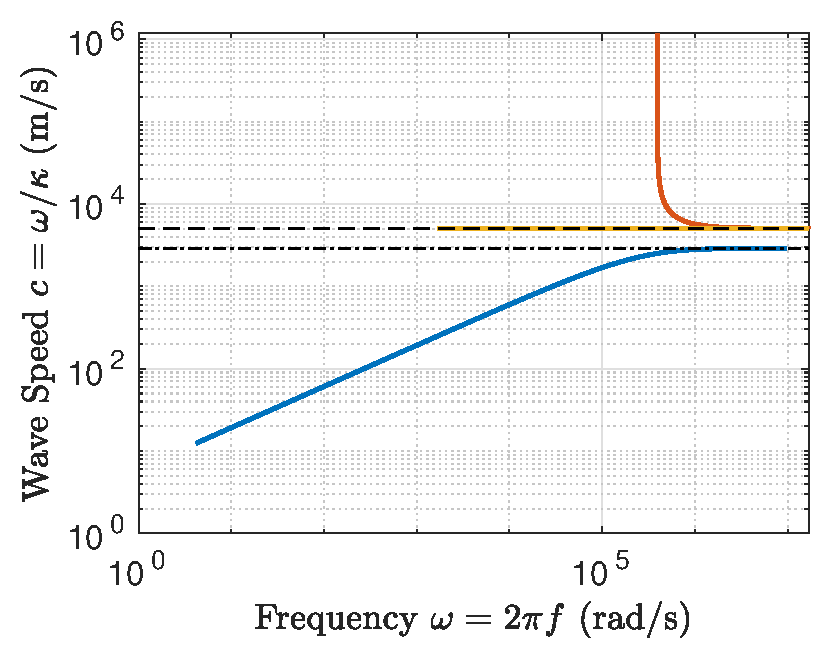
\includegraphics[width=0.35\linewidth]{../../PLANARMODEL/FIGS/TMWS_CvW}
    \end{figure}
  \item Asymptotes corresponding to the case $\omega\to \infty$ are
    depicted using dashed lines in the figure
    \pagebreak
  \item 
  \end{itemize}
\end{frame}

\end{document}
%%% Local Variables:
%%% mode: latex
%%% TeX-master: t
%%% End:
